
\chapter{Quantum measurement and feedback control}
\label{c:qm}

The measurement process in quantum mechanics is as full of surprises and unintuitive conclusions as the rest of quantum theory.  Unlike in classical physics, quantum physics enforces intrinsic limitations in the precision with which certain classes of measurements can be made.  Furthermore, the effect of the measurement process on the system undergoing measurement---the \textit{back-action} of the measurement---is fundamental and unavoidable, and measurements of a quantum system can and will strongly impact the future evolution of the state of that system.

I will begin this chapter by describing two classic thought experiments which help elucidate where quantum limits to measurements arise in an intuitive way.  From this basis, I will discuss several useful categorical distinctions between different types of quantum measurements which will serve to focus the discussion.  This discussion leads to the concept of the \textit{quantum efficiency} of a measurement, needed to describe experiments in which some of the information extracted by a measurement is lost.  I will then discuss the more concrete case of a two-level system undergoing continuous measurement and describe how Bayesian statistics can be employed to reconstruct the full quantum state of the system from a continuous measurement record.  This ability to track the quantum state of the system naturally implies the possibility of attempting to steer the evolution of this state during measurement, leading to a discussion of the quantum feedback control used to stabilize Rabi oscillations of a qubit which will close the chapter.

\section{Two classic thought experiments on quantum measurement}

The examples and discussion in this section follow the seminal text on quantum measurement by Braginsky and Khalili \cite{Braginsky1992}.  This text was my first introduction to the subject; although at this point in time the work is quite dated, it still stands as an excellent introduction to the subject.  In order to understand at an intuitive level where quantum limits on measurements arise, I will reproduce and comment on the discussions of two thought experiments: the \textit{Heisenberg microscope} and the \textit{ponderomotive probe for energy}.

\subsection{The Heisenberg microscope}

\begin{figure*}
\begin{center}
	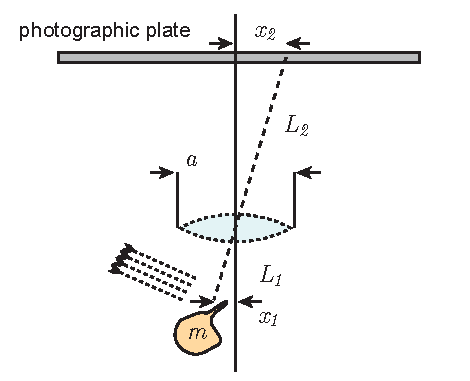
\includegraphics[width = 3.13in]{qmeas_chapter/heismicro}
\end{center}
\caption[Heisenberg microscope]{Heisenberg microscope apparatus.}
\label{fig:heismicro}
\end{figure*}

The Heisenberg microscope is a thought experiment originally described by Werner Heisenberg in 1930 \cite{heisenberg1930physical}.  Although the apparatus described is not at all practical, it does capture all of the critical elements needed to understand the role of the uncertainty principle in the determination of quantum quantities.  Suppose we were interested in attempting to measure the position $x_1$ of a macroscopic object of mass $m$.  We could imagine doing so by scattering some light off of this object and observing the position of the object using a microscope.  The apparatus to do so is shown in Figure \ref{fig:heismicro}.  We imagine attaching a thin rod to the object, whose diameter is less than an optical wavelength.  Presuming we know the approximate position of the object, we can arrange a lens and photographic plate near the object, with the rod close to the focal plane of the lens.  This lens-plate system provides an optical amplification factor of approximately $L_2/L_1$ where $L_1$ is the focal length.

We send in a stream of photons to impinge on the rod, and wait for a single photon to be scattered by the rod, pass through the lens' aperture $a$, and strike the photographic plate, producing a small grain of silver.  The position of this grain $x_2$ can be determined to an accuracy much better than an optical wavelength.  From $x_2$ we can infer the position of the object $x_1 = -x_2 L_1 / L_2$.  However, we cannot make this determination precisely due to the wave nature of light.  The position at which the photon scattered off the rod is not well determined below the spot size of the lens, resulting in an uncertainly in the position
\begin{equation}
\Delta x_{\textrm{measure}} \simeq \frac{1}{2 \pi}\lambda \frac{L_1}{a}.
\label{eq:dxmeas}
\end{equation}
Additionally, because the photon possesses momentum $P = \hbar \omega / c$ and passed through the lens' aperture $a$, it must have transferred to the rod (and thus the attached mass) a random momentum in the $x$ direction with unknown sign and a magnitude on the order of
\begin{equation}
\Delta P_{\textrm{perturb}} \gtrsim \frac{\hbar \omega}{c} \frac{a}{2 L_1} 
\label{eq:dPpert}
\end{equation}
for $a/L_1 \ll 1$.  If we take the product of these two uncertainties, we recover the familiar-looking result
\begin{equation}
\Delta x_{\textrm{measure}} \Delta P_{\textrm{perturb}} \gtrsim \frac{\hbar}{2}.
\label{eq:dxdP}
\end{equation}

This example captures the essential features of any quantum measurement.  We extract information about some observable quantity to within some definite error.  In the process of doing so, we inevitably perturb at least one other quantity of the system---the measurement has some finite \textit{back-action}.  Finally, at some stage of the measurement something \textit{irreversible} occurs (in this case, the measurement photon ceases to exist and a grain of silver is created); this irreversible event is related to crossing the fuzzy boundary between the quantum system under measurement and the classical world we conduct our experiments from.  It is important to note that this \textit{measurement-disturbance} relation is of a fundamentally different nature than the standard position-momentum Heisenberg uncertainty relation, which is the result of the simultaneous measurement of two or more non-commuting quantities.  Here, we only measure one quantity, but the determination of that quantity implies some minimum disturbance to the system under measurement.

One way of understanding the existence of an uncertainty principle for measurement is as an implication of the uncertainty principle applied to the measurement system itself.  Unfortunately, we cannot simply compel a quantum system to reveal its state to us, no matter how loudly we demand it.  By necessity, to measure a quantum system, we must couple that system to some auxiliary system which comprises part or all of a measurement apparatus.  That measurement system itself must also obey the laws of quantum mechanics, which imply that the state of the measurement system must have some finite uncertainty in the preparation of its state.  This uncertainty in the measurement apparatus results in the finite precision of the measurement $\Delta x_{\textrm{measure}}$, and the uncertainty principle then insists that as we reduce the position uncertainty of the object under measurement, the uncertainty in the momentum of the object must increase.

\subsection{The ponderomotive probe for energy}
\label{sec:ponder}

In the case of the Heisenberg microscope, the back-action of the measurement fundamentally influences the future evolution of the quantity we want to determine as the random momentum kick delivered by the photon mixes into the position coordinate through the continued Hamiltonian evolution of the motion of the free mass.  Because of this relationship, if we repeatedly measure the position of the mass by scattering many photons and measuring their displacement, we will not be able to reduce the uncertainty in the position of the free mass to arbitrary precision.  This can be understood as the result of the fact that the eigenstates of the measurement process and the eigenstates of the dynamical evolution of the free mass are not the same.  A state of definite position roughly corresponds to an eigenstate of the measurement.  However, the dynamical evolution of the free mass implies the spreading of a wave packet of definite position.

There is an important class of quantum measurements, called \textit{quantum nondemolition}\footnote{The term quantum nondemolition is perhaps a bit unfortunate and is tangled up with historical ideas of quantum measurements using photons.  Many classes of traditional measurements of quantum systems---for example, detecting photons by absorbing them in a dissipative process such as a photomultiplier tube---literally destroy the system under measurement.  Though physically preserving the system undergoing measurement is a necessary condition for a measurement to be QND, it is hardly sufficient.}
(QND) measurements, that avoid this issue.  If the observed quantity under measurement is itself an eigenstate of the dynamical evolution of the measured system, then reductions in the uncertainty in this quantity will not result in the dynamics of the system mixing the measurement back-action into the measured quantity.
\begin{figure*}
\begin{center}
	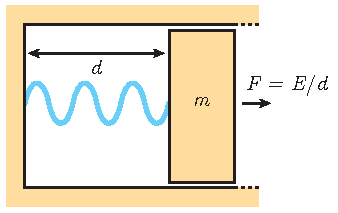
\includegraphics[width = 2.25in]{qmeas_chapter/ponder}
\end{center}
\caption[Ponderomotive probe for energy]{Apparatus for detecting the energy in a cavity resonator by measuring the ponderomotive force on a movable wall.}
\label{fig:ponder}
\end{figure*}
A useful thought experiment that demonstrates all of the important features of a QND measurement is the measurement of the energy in an electrical cavity resonator by measuring the ponderomotive force (i.e. electromagnetic/radiation pressure) that energy exerts on a movable wall of the cavity.  This thought experiment is discussed in Chapter 4 of reference \cite{Braginsky1992}.  A schematic of the setup for this experiment is shown in Figure \ref{fig:ponder}.  We assume that the mass $m$ of the movable wall is large enough that the motion of the wall will be slow compared to the oscillation frequency of the field inside the cavity; in other words, we assume the motion of the wall to be adiabatic.

The ponderomotive force acting on the movable wall of the resonator is $F = E/d$ where $E$ is the resonator's energy and $d$ is a length that is proportional to the size of the resonator and also depends on which resonant mode is excited.  The force $F$ during a measurement of finite time $\tau$ changes the momentum of the wall by $\delta P = E \tau / d$; thus, a measurement of the change in momentum of the wall amounts to a measurement of the energy.  The uncertainty in our determination of the energy of the resonator is proportional to the uncertainty in the initial momentum of the wall, such that
\begin{equation}
\Delta E_{\textrm{measure}} = \frac{d}{\tau} \Delta P.
\label{eq:dEmeas}
\end{equation}
However, the smaller we make the initial uncertainty in momentum, the larger the corresponding uncertainty in the position of the wall $\Delta x$ must be.  An uncertainty in the position of the wall implies an uncertainty in the size $d$ and thus of the resonant frequency of the resonator $\Delta \omega = \omega \Delta x / d$ which in turn produces a random change in the resonator's phase during the measurement
\begin{equation}
\Delta \phi_{\textrm{perturb}} = \Delta \omega \tau = \omega \tau \frac{\Delta x}{d}.
\label{eq:dPhi}
\end{equation}
Combining (\ref{eq:dEmeas}), (\ref{eq:dPhi}), and the uncertainty principle $\Delta x \Delta P \geq \hbar/2$, we obtain the measurement uncertainty relation
\begin{equation}
\Delta E_{\textrm{measure}} \Delta \phi_{\textrm{perturb}} \geq \frac{\hbar \omega}{2}.
\label{eq:dEmeasdPhi}
\end{equation}
We have once again derived an uncertainty relation for the minimum product of our knowledge of the state of the system and the magnitude of the back-action on that system: the more precisely we measure the energy in the resonator, the more uncertain the phase of the oscillation must become.

Unlike in the case of the free particle in the Heisenberg microscope, the observable measured in this experiment (energy) is also a constant of motion of the Hamiltonian of the system under measurement.  The Hamiltonian for the resonator is
\begin{equation}
H = \hbar \omega N
\label{eq:Hres}
\end{equation}
where $N$ is the number of quanta in the resonator.  Eigenstates of the Hamiltonian are of course eigenstates of definite energy, and since the motion of the wall is assumed to be adiabatic, the number of quanta in the resonator does not change.  Thus, by measuring the momentum of the wall for longer and longer times $\tau$ we can reduce the uncertainty in the energy to arbitrary precision.

This measurement possesses all of the properties constituting an ideal quantum measurement.  There is no fundamental constraint on the precision with which we can determine the measured quantity.  Furthermore, the measurement need not itself perturb the quantity under measurement.  The measurement must, however, perturb the quantity which is canonically conjugate to the measured observable in accordance with the uncertainty principle.

\section{Classes of quantum measurements}

In this section I will elaborate some useful distinctions between different classes of quantum measurements.  Specifying which classes of measurements are most relevant to the quantum measurement protocols used in the experiments described in this thesis will serve to focus the remainder of the discussion in the chapter to the theoretical techniques most useful for this subset.

\subsection{Direct and indirect measurements}

Roughly speaking, we can divide any quantum measurement into one of two categories: \textit{direct} and \textit{indirect} measurements.  The difference between the two amounts to where the fuzzy boundary between the classical and quantum worlds is crossed.  In any measurement performed by a laboratory experimenter, some part of the measurement apparatus must obey the laws of classical physics.\footnote{At least, as far as we are presently aware.} The distinction between a direct and indirect measurement is essentially related to how well the quantum system of interest remains safely isolated in the quantum domain.

In a direct measurement, the quantum system undergoing measurement is directly coupled to one or more classical degrees of freedom in the measurement apparatus.  An example of such a measurement is the detection of a photon using a photomultiplier tube.  The arrival of a photon immediately triggers a highly classical cascade of current in the tube, and the quantum system directly sustains any classical back-action from the measurement apparatus (in this case, being completely destroyed).  Since the measurement apparatus is classical and likely contains a large number of degrees of freedom, the back-action of a direct measurement is typically much larger than any minimum bounds set by quantum mechanics.

In contrast to direct measurements, indirect measurements place some auxiliary quantum probe system between the quantum system of interest and the classical measurement apparatus.  The probe system and the main system are brought into contact with one another, allowed to interact for some time, and then decoupled.  The probe system is then brought into contact with the rest of the measurement apparatus, and a direct measurement of the probe is made.  In this way, the excess back-action of the classical measurement is absorbed by the probe system, effectively isolating the main system.  This technique directly permits repeated, minimally-invasive measurements of the main system, using the following procedure.  We first create an ensemble of identically-prepared probe systems.  Each probe system is brought into contact with the main system in series and is then directly measured.  We discard the probe systems after the direct measurement, also discarding the extra back-action of the rest of the measurement apparatus.

There are certain measurements in mesoscopic systems that do not neatly fit into these two categories of direct and indirect measurement.  These are cases where the probe system cannot be described as being firmly classical or firmly quantum.  Even though a measurement may be sensibly described as a direct measurement, the back-action of that measurement may in fact be relatively minimal and non-invasive.  The measurement of a superconducting qubit using a Josephson bifurcation amplifier (JBA) \cite{Vijay2009} is an example of a direct measurement that may not neatly be described as indirect.  The operating principle of the JBA is based on the physics of a nonlinear oscillator; when driven with a very strong drive near the resonant frequency, the dynamics of the oscillator bifurcate into two stable states of very different oscillation amplitude which are quite classically distinguishable.  Moreover, it is not known if the process of switching between these states is reversible or not.  Several experiments \cite{Lupascu2007,Boulant2007} have been performed on this measurement process and have determined that the back-action may be relatively gentle for a measurement which could be considered a direct measurement.

For the remainder of this chapter I will focus exclusively on measurements that fall into the category of indirect measurements.

\subsection{Quantum nondemolition measurements}

Virtually all of the measurements described in the main results of this thesis are quantum nondemolition measurements.  As such, it is important to briefly describe a precise and pleasingly concise definition of the requirements on a measurement process for the measurement to be QND.  The ponderomotive energy probe described in section \ref{sec:ponder} introduced a rough qualitative definition of a QND measurement, namely, that the state of the system corresponding to increasing measurement precision must also correspond to a dynamically stable state of the system's Hamiltonian.  In this section I introduce the most generally used criterion for a measurement to be QND, following the discussion in Chapter 4 of reference \cite{Braginsky1992}.

If we measure some generic observable quantity $q$ of a quantum system, and express the action of the measurement as an operator $U$ which acts on the joint state of the system under measurement and the probe system, we require that the measurement not perturb the quantity undergoing measurement; that is, we require the evolution operator to commute with the measured quantity:
\begin{equation}
[q,U] = 0.
\label{eq:QNDfullsys}
\end{equation}
In other words, the operator $U$ corresponds to the operator for the system we would compute by solving for the full Hamiltonian evolution in time of the coupled system over the entire measurement interval.  This task is in general quite non-trivial, so a slightly less general and more stringent condition for defining a QND measurement is normally used.  Namely, that the Hamiltonian describing the joint evolution of the system and the probe commutes with the measured observable,
\begin{equation}
[q,H_{\textrm{tot}}] = 0.
\label{eq:QNDHtot}
\end{equation}
This condition is more stringent than (\ref{eq:QNDfullsys}), as it implies that $q$ does not change at any point during the measurement, while (\ref{eq:QNDfullsys}) implies that $q$ can evolve during the measurement period but that by the end of the measurement it has returned to its original value.

We can further simplify this criteria by expressing $H_{\textrm{tot}}$ in the very general form
\begin{equation}
H_{\textrm{tot}} = H_{\textrm{obj}} + H_{\textrm{probe}} + H_{\textrm{int}}
\label{eq:Htot}
\end{equation}
where $H_{\textrm{obj}}$ and $H_{\textrm{probe}}$ are free evolution Hamiltonians of the measured system and the probe, respectively, and $H_{\textrm{int}}$ is their interaction Hamiltonian.  Since $q$ is an observable of the measured system and not the probe,
\begin{equation}
[q,H_{\textrm{probe}}] = 0.
\label{eq:qHprobe_com}
\end{equation}
If we assume that $q$ is a constant of motion of $H_{\textrm{obj}}$, then
\begin{equation}
i \hbar \frac{\partial q}{\partial t} +  [q,H_{\textrm{obj}}] = 0.
\label{eq:q_const_motion}
\end{equation}
If $q$ has no explicit time dependence, $\frac{\partial q}{\partial t} = 0$, and by combining (\ref{eq:QNDHtot}), (\ref{eq:qHprobe_com}), and (\ref{eq:q_const_motion}), we arrive at the most common and illuminating definition for a measurement to be QND:
\begin{equation}
[q,H_{\textrm{int}}] = 0.
\label{eq:QND_cond}
\end{equation}
For the remainder of this chapter, I will focus the discussion on measurement theory relevant to QND measurements.

\subsection{Discrete and continuous quantum measurements}

In any physical realization of a quantum measurement, the measurement process will occur over some finite time scale.  This time scale could be the duration of the interaction between the probe system and the main system in an indirect measurement, for example, which results in a single measurement outcome.  We could also imagine a case where we perform many indirect measurements in rapid succession and the cumulative duration of all of these measurements constitute the measurement time scale, compounding the results of all the measurements into a single outcome.  In this latter case, we could also imagine considering the stream of serial measurements as producing a time series of measurement outcomes.  As we continuously integrate these individual measurements, our knowledge of the quantity being measured improves.  Alternatively, we could consider this time series of measurement outcomes as describing a record of the evolution of the measured observable during the measurement period, presuming we have some information about the value of that observable at the beginning of the measurement.

The primary distinction between a discrete measurement and a continuous measurement is essentially a matter of interpretation.  A discrete measurement, resulting in a single estimate of the quantity under measurement, can also be constructed as the integration of a continuous measurement over some finite time to produce a single value.  A continuous measurement can also then be constructed as the continuous limit of a series of rapid discrete measurements performed on a time scale much faster than the evolution time of the quantity being measured.  The measurements comprising the experimental results of this thesis fall into both of these categories.

\section{Ideal and imperfect projective measurements}

The standard textbook description of a quantum measurement involves the instantaneous transition of the quantum state of the measured system from an arbitrary superposition state into a single eigenstate of the measured operator.  The action of the measurement is thus to ``magically'' coerce the system into the joint eigenbasis of the measurement operator and the system.  Repeated textbook measurements yield the same eigenvalue for all measurements after the first measurement.  This process is assumed to be perfect, and always yields a single eigenvalue with certainty, though which eigenvalue is non-deterministic and probabilistically depends on the square of the corresponding eigenvector component of the state vector.

\begin{figure*}
\begin{center}
	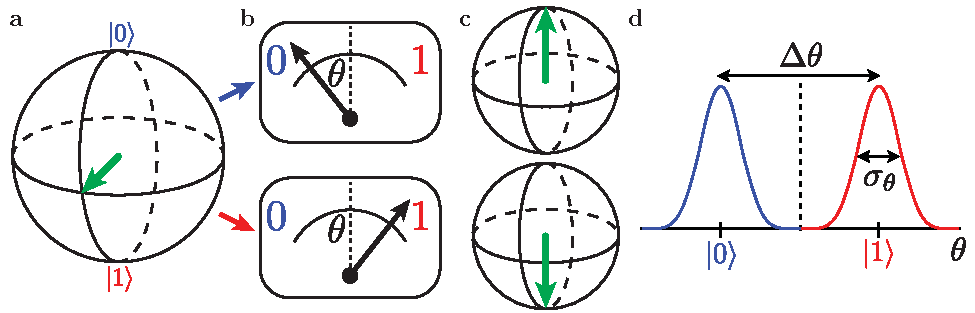
\includegraphics[width = 6.5in]{qmeas_chapter/ideal_proj_meas}
\end{center}
\caption[Ideal projective measurement]{Thought-experimental protocol for an ideal projective measurement. \textbf{a} Bloch sphere representation of a qubit initially prepared in the equal superposition state $(|0\rangle + |1\rangle)/\sqrt{2}$. \textbf{b} An ideal projective measurement is made of the state of the qubit, swinging a classical meter to either the state 0 or 1. \textbf{c} The state of the qubit after the measurement is made is the eigenstate corresponding to the measurement outcome.  \textbf{d} Histogram of many iterations of the thought experiment, showing probability distributions for the angular coordinate of the classical meter.  The finite width of each histogram $\sigma_\theta$ is the result of unavoidable quantum or classical fluctuations of the measurement apparatus.  So long as the separation $\Delta \theta$ is much greater than the histogram width, we can unambiguously map the qubit state to the angular coordinate of the meter, and the measurement is still ideal.}
\label{fig:ideal_proj_meas}
\end{figure*}

It is useful to formulate a picture of an ideal projective measurement for a more realistic case than the straightforward textbook definition.  To simplify the discussion, I will specifically discuss the case of the ideal projective measurement of a two-state quantum system (a qubit).  For some initial coherent qubit state
\begin{equation}
|\Psi\rangle = \alpha |0\rangle + \beta |1\rangle
\label{eq:qubit_psi}
\end{equation}
where $\alpha$ and $\beta$ are complex amplitudes with the normalization condition $|\alpha|^2 + |\beta|^2 = 1$, an ideal projective measurement of the qubit returns the eigenvalue 0 with probability $|\alpha|^2$, and the eigenvalue 1 with probability $|\beta|^2$.  Furthermore, the qubit state following the measurement should be the eigenvector corresponding to the measured eigenvalue.

Without introducing any technical details about the exact nature and form of the overall measurement apparatus, we can construct a fairly general picture of what it means in practice to realize an ideal measurement.  An outline of this measurement is shown in Figure \ref{fig:ideal_proj_meas}.  I will assume that the measurement apparatus is sufficiently precise and optimal to realize a perfect QND measurement with no excess back-action.  The output of the measurement is the angular deflection of a classical, continuous, one-dimensional meter, with two states labelled 0 and 1.

If we repeatedly prepare some initial qubit state---for example, the equal superposition state $|\Psi\rangle = (|0\rangle + |1\rangle)/\sqrt{2}$---and then histogram the results of each measurement, we will recover a set of histograms that look something like the plot shown in Figure \ref{fig:ideal_proj_meas}d.  The histograms corresponding to each state will in general have some finite width due to intrinsic fluctuations (be they classical or quantum) in the measurement apparatus; so long as these fluctuations are significantly smaller than the separation between the histograms, we can unambiguously map the qubit states $|0\rangle$ and $|1\rangle$ onto the meter states 0 and 1.

\begin{figure*}
\begin{center}
	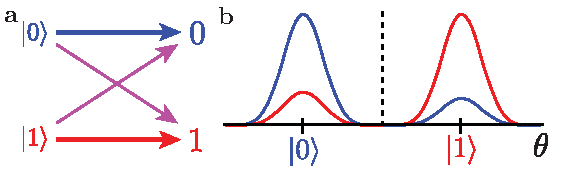
\includegraphics[width = 3.75in]{qmeas_chapter/proj_state_map}
\end{center}
\caption[Projective measurement error due to state mapping]{\textbf{a} Diagram showing the possible permutations of mappings between qubit and meter states, including the error terms in purple. \textbf{b} Ideal measurement histograms, showing the effect of the state mapping errors on measured histograms for the qubit states.}
\label{fig:proj_state_map}
\end{figure*}


Real quantum measurements can deviate from this ideal behavior in a variety of different ways, essentially corresponding to the ways in which the transitions between the panels of Figure \ref{fig:ideal_proj_meas} can go wrong.  First, the mapping between the qubit and meter states could involve non-idealities, schematically shown in Figure \ref{fig:proj_state_map}.  This type of error could be due to some fundamental limitation in the measurement technique which does not produce the ideal state map, thus leaving the qubit and meter in an inconsistent configuration (this fundamentally makes the measurement not perfectly QND).  This type of error could also be the result of imperfections which are not fundamental to the measurement process itself, such as undesired state transitions in the qubit during the measurement, which may or may not leave the qubit and meter in an inconsistent state.

\begin{figure*}
\begin{center}
	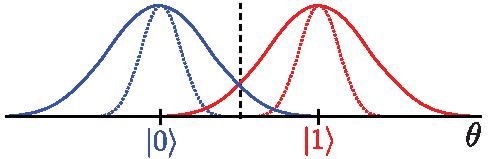
\includegraphics[width = 3.25in]{qmeas_chapter/proj_meas_noise}
\end{center}
\caption[Projective measurement error due to noise]{If the measurement apparatus is noisy, the measurement histograms may be broadened.  If this broadening is large enough to make the histograms overlap, a clear distinction between meter states is no longer possible, introducing a measurement error in the overlap region and possibly making the meter state inconsistent with the qubit state.}
\label{fig:proj_meas_noise}
\end{figure*}

Second, the measurement apparatus itself may be of poor quality and not satisfy the requirement that $\Delta \theta \gg \sigma_\theta$, resulting in measurement histograms that partially overlap, as shown in Figure \ref{fig:proj_meas_noise}.  This type of error is assumed to be entirely related to the function of the measurement apparatus, such that the extra measurement uncertainty is uncorrelated with any quantum measurement uncertainty in the state measurement itself.

Overall, the extent to which a projective qubit measurement accurately captures the quantum state is called the \textit{measurement fidelity}, and is defined based on the action of the measurement on a qubit prepared in one or the other eigenstate.  The fidelity is defined as
\begin{equation}
F = 1 - P(1|0) - P(0|1)
\label{eq:ro_fid}
\end{equation}
where $P(i|j)$ is the probability that the measurement apparatus returned the state $i$ when the qubit was prepared in the state $j$.  A perfect measurement with no errors corresponds to a fidelity of unity.  The worst possible assignment of states in a measurement would be fully random, where $P(0|1) = P(1|0) = 0.5$ and thus $F = 0$.

\section{Ideal and imperfect partial measurements}

Consider for a moment the ideal projective measurement process depicted in Figure \ref{fig:ideal_proj_meas}.  Suppose we have mastered the theory of quantum measurement and we have designed a qubit measurement apparatus that we are very convinced is ideal.  We know for a fact that it performs a QND measurement, applies no excess back-action to the qubit, and the noise in the measurement apparatus is completely limited by minimum bounds set by quantum mechanics.

\begin{figure*}
\begin{center}
	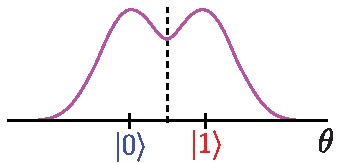
\includegraphics[width = 2.25in]{qmeas_chapter/ideal_partial_meas}
\end{center}
\caption[Partial measurement histograms]{Histogram of the output of the classical meter for an ideal measurement of an ensemble of identically prepared qubit equal superposition states.  The histogram overlap in this case is only due to fundamental quantum fluctuations of the measurement system, not added classical noise.}
\label{fig:ideal_partial_meas}
\end{figure*}

We prepare the qubit in the equal superposition state $|\Psi\rangle = (|0\rangle + |1\rangle)/\sqrt{2}$ and then make a single measurement.  We repeat this state preparation many times, histogramming the results of all of the measurements, resulting in the histogram shown in Figure \ref{fig:ideal_partial_meas}.  Because we have assumed that the measurement apparatus adds no classical noise, this case does not correspond to the noise-broadened projective readout distributions shown in Figure \ref{fig:proj_meas_noise}.  How are we to interpret this distribution?  Moreover, how are we to interpret the outcome of any of the single measurements that make up this distribution?  The answers to these questions lie beyond the textbook definition of quantum measurement.

The measurement just described constitutes a \textit{partial quantum measurement} (sometimes called a \textit{weak quantum measurement}).  Since the histograms for the $|0\rangle$ and $|1\rangle$ states at least partially overlap, we cannot precisely determine which eigenstate the qubit has been projected into.  However, since the overlap is exclusively due to the quantum fluctuations of the measurement apparatus, this uncertainty in the state determination is not merely the result of our crude, classical ineptness---no observer in the universe is able to completely determine that the qubit has been projected into one or the other eigenstate, and, thus, it hasn't been completely projected at all!

The state of the qubit has, in fact, evolved as a result of the measurement, in some manner consistent with the measurement outcome (just as in a projective measurement).  However, unlike in a perfect projective measurement, we are now faced with a continuum of possible measurement outcomes, where each possible value is correlated with a particular measurement back-action on the qubit state.  For a projective measurement, this back-action is the usual act of projecting the qubit into the eigenstate consistent with the meter outcome.  To determine the equivalent mapping between this new continuous spectrum of meter outcomes and the resulting back-action, we will need to first develop some statistical tools.

It could of course be possible that all of the histogram overlap is not due to the intrinsic quantum fluctuations of the measurement apparatus.  If some of the overlap is due to additional classical noise in the measurement, as in Figure \ref{fig:proj_meas_noise}, we cannot disentangle the added fluctuations from the intrinsic fluctuations and our measurement is no longer perfect.  In this case, we will not be able to create an ideal mapping between measurement outcomes and back-action on the qubit, but rather some of this back-action must be expressed as a decrease in the purity of the ensemble qubit state as a result of the measurement.  The quality of a measurement apparatus in this case is described by a \textit{quantum efficiency} $\eta$, where $\eta$ is qualitatively given as the ratio of the size of the quantum fluctuations to the size of the total fluctuations in the measurement apparatus.  This concept will be made more concrete shortly.



\subsection{Quantum Bayesian inference}\label{s:bayesian}

Partial quantum measurements, where we acquire some finite and incomplete information about the state of a quantum system from a measurement, are a natural fit for analysis using Bayesian statistics.  We start with some initial estimate of the density matrix describing the system under measurement; if we have no initial information, this density matrix will be essentially a maximum-entropy placeholder.  We perform a partial measurement, and then use the result of that measurement to update our best estimate of the new density matrix conditioned on the measurement outcome.  If we have realized a perfect quantum measurement apparatus, then the measurement outcome should perfectly correlate with the coherent evolution of the density matrix as a result of the measurement, enabling the perfect tracking of a known initial state.

The quantum Bayesian (QB) approach \cite{qu_bayes,koro11} is relatively modern compared to other more traditional theoretical frameworks for understanding partial measurements such as positive operator-valued measures (POVM) .  The QB approach has the advantage of being relatively straightforward to calculate compared to POVMs, and I personally find it to provide more illuminating insight into how our state of knowledge evolves as the result of a partial measurement.  All of the experimental results described in this thesis are well modeled in the QB framework, and as such I will not explicitly discuss POVMs but rather refer to a excellent treatment on the subject for further reading \cite{jaco06}.

If we presume that we begin the experiment described in Figure \ref{fig:ideal_partial_meas} with an ensemble of qubits identically prepared in the state $|\Psi\rangle = (|0\rangle + |1\rangle)/\sqrt{2}$, we can describe the state of that ensemble with the density matrix
\begin{equation}
\rho(t=0) = \frac{1}{2} \left( \begin{array}{cc}
1 & 1 \\
1 & 1 \end{array} \right)
\label{eq:rho_equal}
\end{equation}
in the $\sigma_z$ basis.  The diagonal entries in this matrix represent the classical probability for finding the system in one or the other eigenstate, while the off-diagonal elements indicate the extent to which the ensemble exists in a superposition of eigenstates.  Because the diagonal elements can be naturally interpreted as classical probabilities, we can apply Bayes' rule to update these values following a partial measurement, calculating the probability to find the qubit in one or the other eigenstate conditioned on the Bayesian estimate of that probability.  Bayes' rule captures the essential procedure for updating our state of knowledge of a system based on some new (incomplete) piece of information acquired about that system:
\begin{equation}
P(A|\beta) = \frac{P(\beta|A) P(A)}{P(\beta)}
\label{eq:bayes_rule}
\end{equation}
where the conditional probability to find the system in the state $A$ given some new measurement result $\beta$ is equal to the probability of having gotten the outcome $\beta$ if the state is in fact $A$ multiplied by our current best estimate for the probability of the system being in the state $A$.  The denominator is a normalization factor.

In the measurements described in this thesis, the coordinate that represents the output of our classical meter will be a voltage $V$ rather than an angle $\theta$, so I will use $V$ for consistency.  Applying \ref{eq:bayes_rule} to the situation at hand results in the following update to the density matrix diagonal elements following a measurement which produces the outcome $V$:
\begin{equation}
P(i|V) = \rho_{ii}(t) = \frac{P(V|i)P(i)}{P(V)}
\label{eq:Pi_update}
\end{equation}
where $P(i)$ is the probability to measure the state $|i\rangle$, given by $\rho_{ii}(t=0)$, and $P(V)$ is the probability to have observed the measured outcome $V$, given by a weighted prior probability distribution conditioned on our knowledge of the initial state $\rho$ and the distribution of measurement outcomes for the states 0 and 1 ($P(V)$ is the distribution plotted in Figure \ref{fig:ideal_partial_meas}).  If we assume that the probabilities of measuring a particular value $V$ when the qubit is prepared in the ground or excited state are normalized Gaussian distributions of width $\sigma$ centered around $\pm \Delta V/2$,  then
\begin{align}
\rho_{11}(t) &= \frac{\rho_{11}(0)}{P(V)}  \exp {\left( \frac{-(V - \Delta V/2)^2}{2\sigma^2} \right)} \label{eq:Pi_update_gauss_11} \\
\rho_{00}(t) &= \frac{\rho_{00}(0)}{P(V)}  \exp \left( \frac{-(V + \Delta V/2)^2}{2\sigma^2} \right)
\label{eq:Pi_update_gauss_00}
\end{align}
where $P(V)$ is given by our prior knowledge of the qubit state
\begin{equation}
P(V) = \rho_{00}(0)  \exp{\left( \frac{-(V + \Delta V/2)^2}{2\sigma^2} \right)} + \rho_{11}(0) \exp{\left( \frac{-(V - \Delta V/2)^2}{2\sigma^2} \right)}
\end{equation}
and the width $\sigma$ is assumed to be the result of averaging a white noise background with power spectral density $S$ for the measurement time $t$ such that $\sigma^2 = S/2t$ \cite{koro11}.

We can now interpret the experimental distribution from Figure \ref{fig:ideal_partial_meas}.  With $\rho_{00}(0) = \rho_{11}(0) = 1/2$, $P(V)$ is the equally weighted sum of the two Gaussian distributions.  If the measurement value $V$ is exactly equal to 0, $P(V)$ is equal to the exponential term in \eqref{eq:Pi_update_gauss_11} and $\rho_{11}(t) = \rho_{11}(0)$.  Remarkably, in this case, we have made a partial measurement of the state of the qubit which has provided us with \textit{exactly zero information} about which state it is in!  Because we have learned nothing new about the state, there should be no corresponding back-action due to this measurement, reflected in the fact that the density matrix elements have not changed.

If $V>0$, the exponential term in \eqref{eq:Pi_update_gauss_11} will be larger than the exponential term in \eqref{eq:Pi_update_gauss_00}, so $\rho_{11}(t) > \rho_{11}(0)$.  In other words, because this value of $V$ corresponds to an outcome which is more likely if the qubit is in the excited state, the back-action of the measurement must have kicked the state towards $\ket{1}$.  Also note that if $\rho_{ii}(0) = 1$, $\rho_{ii}(t) = 1$ regardless of the measurement outcome.  This is exactly what we expect for a QND measurement: if the qubit is in an eigenstate, the back-action of the measurement should not disturb this eigenstate.  Furthermore, a repeated measurement of an initial superposition state will eventually drive the qubit into one or the other eigenstate, realizing a projective measurement.

If the only back-action of the measurement process is the evolution of the qubit towards one of its eigenstates (leaving the phase of the qubit state unchanged), and we have realized an ideal measurement, then the resulting change in the off-diagonal elements of the density matrix must be completely specified by the change in the diagonal elements:
\begin{equation}
\rho_{01}(0) = e^{i\phi} \sqrt{\rho_{00}(0) \rho_{11}(0)} \quad \rho_{01}(t) = e^{i \phi} \sqrt{\rho_{00}(t) \rho_{11}(t)} 
\end{equation}
implying
\begin{equation}
\rho_{01}(t) = \rho_{01}(0) \frac{ \sqrt{ \rho_{00}(t) \rho_{11}(t)} } { \sqrt{ \rho_{00}(0) \rho_{11}(0)} }.
\label{eq:rho01_update}
\end{equation}
This Bayesian state update procedure and the resulting ability to track a qubit state undergoing measurement has been extensively tested experimentally at QNL \cite{Weber2014,murch_observing_2013,Weber2014a}, demonstrating excellent agreement with theoretical predictions.

It might seem unintuitive at first that we can write down such a simple and seemingly deterministic set of equations for the evolution of the qubit state as the result of a measurement.  The measurement result $V$ is of course still stochastic and unpredictable; however, because we have presumed a perfect, quantum-limited measurement apparatus, and we begin with a known density matrix, the purity of the qubit state need not change as a result of the measurement as no information about the qubit state has been lost or discarded.  Thus, the back-action on the qubit state is perfectly correlated with the measurement result, and the only effect of quantum uncertainty is the unpredictable nature of which measurement result we find.

The ensemble dephasing rate associated with this measurement process, obtained by averaging \eqref{eq:rho01_update} \cite{koro11}, is
\begin{equation}
\Gamma = \frac{(\Delta V)^2}{4S}.
\label{eq:bayesian_dephasing}
\end{equation}
The term ``dephasing'' here is something of a misnomer, as we just asserted that the action of this measurement does not change the phase of a superposition state.  In the ensemble picture, the stochastic evolution of a superposition state towards one of the eigenstates is indistinguishable from stochastic evolution of a superposition state around the equator of the Bloch sphere, so this process is still called dephasing.  At the level of a particular measurement, however, the two processes are fundamentally different, as we will see in a specific example in section \ref{s:cQED_backaction}.  This rate can also be naturally interpreted as the ``strength'' of a measurement; a stronger measurement projects a superposition state into an eigenstate more rapidly, and thus the apparent ensemble dephasing rate is larger.

Remarkably, this fairly straightforward picture actually corresponds very closely to the quantum measurements realized in this thesis.  The primary departure from this idealized picture is that the measurements are not entirely perfect, but rather involve some finite information collection efficiency $\eta < 1$.  This loss of information looks exactly like an extra dephasing of the qubit state characterized by a rate $\gamma$ which depends on $\eta$ and other factors specific to a particular measurement apparatus; to include this effect we simply multiply (\ref{eq:rho01_update}) by an exponentially decaying term $e^{-\gamma t}$ and add $\gamma$ to the right side of \eqref{eq:bayesian_dephasing}.  We can write a simple functional form for the efficiency as
\begin{equation}
\eta = \Gamma_m / \Gamma_{\rm tot}
\label{eq:eta_basic_form}
\end{equation}
where $\Gamma_m$ is the ideal dephasing rate associated with a perfect quantum measurement, while $\Gamma_{\rm tot}$ is the total dephasing measured in a given experiment.  A perfect quantum measurement thus corresponds to $\Gamma_{\rm tot} = \Gamma_m$; additional dephasing from other sources (be it imperfect information collection or dephasing intrinsic to the non-ideal quantum system itself) increases $\Gamma_{\rm tot}$ and thus reduces $\eta$.

\section{Continuous quantum feedback control}

With the Bayesian framework in place to track the evolution of a quantum state undergoing measurement, we can consider utilizing the record of this evolution to actively steer the state towards some desired value using feedback. The basic idea of feedback control is predicated on the assumption that we can measure the state of a system precisely, compare that state to some desired target state, and use our measurement to condition a control signal to steer the system towards the desired state and stabilize it against disturbances.  In classical feedback control this process is relatively straightforward, as our measurement of the system need not disturb the state of that system.  In quantum feedback control, this assumption is fundamentally violated by the measurement-disturbance relations which have been the subject of much of the rest of this chapter.

\begin{figure*}
\begin{center}
	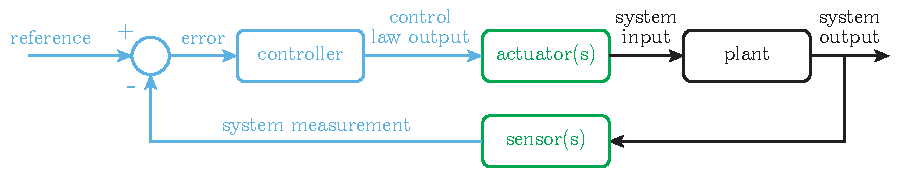
\includegraphics[width = 6in]{qmeas_chapter/feedback_diagram}
\end{center}
\caption[Generic feedback control system]{Block diagram of a generic feedback control system.  The control portion of the system is drawn in blue, the interface between the control and the plant in green, and the plant itself in black.}
\label{fig:feedback_diagram}
\end{figure*}

A generic diagram of a feedback control scheme is shown in Figure \ref{fig:feedback_diagram}.  Consider a system (usually called the \textit{plant}, in a reference to the broad industrial applicability of feedback control) with one or more \textit{sensors} which measure some outputs of the system.  The sensor outputs are subtracted from some \textit{reference} values, producing an error signal that parameterizes the difference between the target state of the system and the current state of the system.  This error is fed into a \textit{controller} which applies some \textit{control law} to the error signal, producing a set of control signals which are fed to one or more \textit{actuators} which apply the control signals to the plant.  Some generic questions control theory asks and answers about this type of system are, for instance, is a particular control law unstable, stable for some parameters, or unconditionally stable?  What control law provides the best control performance, and can a particular control law be shown to be \textit{optimal} in some sense?

In classical control theory, there is no fundamental reason that the precision with which a property of the plant is measured should be of relevance to the dynamical evolution of the plant.  There may be unavoidable noise in the measurements of the plant, but increasing the strength of a measurement should have no result besides increasing the size of the signal relative to this noise.  In quantum measurement, performing a stronger measurement inevitably increases the disturbance on the plant.  Therefore, quantum control theory is faced with additional complexity in analyzing the performance of control laws, especially with regards to optimality.  Measuring a system more strongly may increase the disturbance to such a level that the resulting fluctuations are beyond the ability of the actuators to compensate, for example.  Explicit details on the general methods of quantum control are beyond the scope of relevance for this thesis; see reference \cite{qmcontrol_book} for further reading on the subject.

Besides the additional theoretical complexity of the measurement-disturbance tradeoff, demonstrating quantum feedback control is a significant technological challenge.  We require a system which implements a nearly ideal, variable strength partial quantum measurement, as we will be interested in assessing theoretical items of interest such as the measurement strength which produces optimal control.  If the aim of our feedback control is, for example, the stabilization of an arbitrary qubit state, a projective measurement would immediately destroy the stabilized state.  Experimental systems that meet this demand have only recently been realized, and as such the first two demonstrations of quantum feedback control did not occur until 2011: the stabilization of photon number states in a microwave cavity \cite{haroche_fb}, and the experiment described in this thesis.

\subsection{Stabilization of Rabi oscillations of a qubit}

I will not attempt to lay out some general framework in which to pose the particular quantum control experiment realized in this thesis; I will instead launch into specifics.  The plant will be a qubit described by a density matrix $\rho(t)$, and our control law will aim to stabilize the dynamics of the density matrix in the presence of dephasing.  Specifically, we will continuously drive Rabi oscillations of the qubit and aim to stabilize the phase of these oscillations.  Without yet going into details of the experimental implementation, the sensor output corresponds to a continuous partial measurement of $\langle \sigma_z \rangle$.  The actuator will correspond to the frequency at which we drive Rabi oscillations $\Omega_r$; to correct the phase of the qubit oscillations, we briefly adjust $\Omega_r$ to speed or slow the oscillations.  Our reference signal will be a high-quality classical oscillator oscillating at a target frequency $\Omega_0$, and the error signal will be the phase difference between this reference and the measured phase of the oscillations of $\langle \sigma_z \rangle$.  This setup can be intuitively thought of as a phase-locked loop, though here we are stabilizing the phase of a quantum oscillator.

The theory for this control scheme was formulated by Korotkov in reference \cite{korotkov_dir_fb}.  It is worth nothing that this work was published in 2002 yet it took another 9 years for quantum measurement technology to advance sufficiently to realize it.  My discussion here will more closely follow the discussion in our publication on the experiment \cite{vijay_stabilizing_2012}; specifically, section IV of the supplementary materials.

We will first consider the case where the detector is ideal ($\eta=1$). The qubit evolution during the process of continuous measurement can be described using stochastic equations \cite{Korotkov2001} for the qubit density matrix $\rho$. Stochastic equations are required because the measurement outcome $V(t)$ will fundamentally involve a random variable corresponding to the quantum fluctuations of the measurement apparatus; these expressions are essentially the result of taking the time derivatives of (\ref{eq:Pi_update_gauss_11}) and (\ref{eq:Pi_update_gauss_00}).   The measurement output signal $V(t)$ is given by
\begin{equation}
V(t) = \frac{\Delta V}{2} [\rho_{11}-\rho_{00}] + \xi_{\mathrm{id}}(t)
\label{meas_I}
\end{equation}
where $\xi_{\mathrm{id}}$ is the white noise of an ideal detector characterized by the (one-sided) spectral density $S_{\mathrm{id}}$.  The strength of the measurement, characterized by the measurement induced dephasing rate \eqref{eq:bayesian_dephasing}, is given by
\begin{equation}
\Gamma_{\varphi}=\frac{(\Delta V)^{2}}{4S_{\mathrm{id}}}.
\end{equation}
For a resonant Rabi drive, the stochastic equations describing the evolution of the density matrix under simultaneous driving and measurement (in Stratonovich form) are given by
\begin{equation}
 \dot{\rho}_{11}=-\dot{\rho}_{00}=-\Omega _{\mathrm{R}}\mathrm{Im}\rho_{01}+\rho _{11}\rho _{00}\frac{2\Delta V}{S_{\mathrm{id}}}V(t)-\Gamma_{1} \rho_{11},  \label{Bayes_11}
\end{equation}
\begin{equation}
\dot{\rho}_{01} =i\frac{\Omega _{\mathrm{R}}}{2}\left( \rho _{11}-\rho_{00}\right) -\frac{\Delta V}{S_{\mathrm{id}}}\rho _{01}\left( \rho _{11}-\rho_{00}\right) V(t) -(\Gamma _{\mathrm{env}} + \frac{\Gamma_{1}}{2})\rho _{01},  \label{Bayes_01}
\end{equation}
where $\Gamma _{\mathrm{env}}$ is the environmental dephasing rate and $\Gamma_{1}$ is the qubit energy relaxation rate \cite{korotkov_dir_fb}.

The terms in \eqref{Bayes_11} can be understood as follows.  The first term describes the deterministic state rotation due to the Rabi drive.  The second term describes the stochastic back-action of the measurement on the qubit state.  The prefactor $\rho_{00}\rho_{11}$ is maximal when $\rho_{00} = \rho_{11} = 1/2$, and decreases to zero when either term is zero.  Thus, the measurement has no effect if the qubit is already in an eigenstate, exactly what we expect for a QND measurement.  Otherwise, the measurement stochastically drives the state towards one or the other eigenstate.  The third term models spontaneous energy relaxation from the excited state to the ground state.  The terms in \eqref{Bayes_01} are similar.  Note that the factor $( \rho _{11}-\rho_{00})$ enforces the evolution described by \eqref{eq:rho01_update}.  The third term describes the decoherence of the state due to both intrinsic environmental dephasing $\Gamma_{\rm env}$ and energy relaxation $\Gamma_1$.

To obtain a closed form expression for the action of feedback control, it is possible to reduce the number of qubit degrees of freedom down to only one.  First, because a resonant Rabi drive rotates the qubit about the $x$-axis and our measurement does not alter the phase of a superposition state, the qubit state is restricted to the $x=0$ plane. Second, by neglecting energy relaxation, we can consider the qubit state as pure, ascribing any measurement inefficiency ($\eta<1$) to some additional noise at the detector output \cite{Kor-nonideal}.  We set $\Gamma_{\rm env}=0$ in equation (\ref{Bayes_01}) and model both environmental dephasing and detector inefficiency by adding a noise term $\xi_{\mathrm{add}}(t)$ to equation (\ref{meas_I}), resulting in the measurement outcome
\begin{equation}
V(t) = \frac{\Delta V}{2} [\rho_{11}-\rho_{00}] + \xi_{\mathrm{id}}(t) + \xi_{\mathrm{add}}(t),
\label{meas_I_analytic}
\end{equation}
where $\xi_{\mathrm{add}}(t)$ has a spectral density $S_{\mathrm{add}} = S_{\rm out} - S_{\rm id}$, where $S_{\rm out} = S_{\rm id}/\eta$ is the total output noise. Therefore, the qubit state evolution can be described by only one parameter, the polar (zenith) angle $\theta(t)$ on the Bloch sphere:
\begin{equation}
\xpec{\sigma_z}(t)= \cos [\theta(t)], \,\,\, \xpec{\sigma_y}(t)=\sin[\theta(t)], \,\,\, \xpec{\sigma_x}(t)=0.
\end{equation}

The goal of the feedback is to stabilize the Rabi oscillation to the form $\theta(t)=\Omega_0 t$ with a fixed frequency $\Omega_0$. We characterize the feedback efficiency $D$ \cite{korotkov_dir_fb} as
\begin{equation}
D=\overline{\cos [\theta_{\rm err}(t)]}, \,\,\, \theta_{\rm err}(t) = \theta(t)-\Omega_0 t,
\end{equation}
which corresponds to the time-averaged scalar product of the desired and actual state vectors on the Bloch sphere.  The qubit ``phase shift error'' $\theta_{\rm err}$ evolves as \cite{korotkov_dir_fb}
\begin{equation}
\dot\theta_{\rm err} = -\frac{\Delta V}{S_{\rm id}} \sin \theta \left(\frac{\Delta V}{2}\cos \theta +\xi_{\rm id}\right).
\label{evol}
\end{equation}
In order to compensate this dephasing-induced phase shift, we now apply feedback by modulating the frequency of the Rabi drive with a feedback term $\Omega_{\rm fb}(t)$ as
\begin{equation}
\Omega_{\rm R}(t) =\Omega_0+\Omega_{\rm fb} (t).
\label{fb0}
\end{equation}
The control law is a simple proportional control, which Korotkov refers to as the ``direct feedback'' control law:
\begin{equation}
\frac{\Omega_{\rm fb}(t)}{\Omega_0} = F \frac{4}{\Delta V} \,\sin (\Omega_0 t) V(t - \tau_{\rm delay}).
\label{fb}
\end{equation}
Here $F$ is the dimensionless feedback gain and the choice of the normalization factor $4/\Delta V$ corresponds to $\Omega_{\rm fb}/\Omega_0=-F\sin\theta_{\rm err}$ on average.  The extra term $\tau_{\rm delay}$ in the argument of $V$ accounts for the fact that in general our measurement and feedback control will have some finite bandwidth, so that the control correction we apply to the system at time $t$ actually corresponds to a measurement made at some earlier time, delayed by $\tau_{\rm delay}$.  For the moment we assume this delay to be negligibly small.

The qubit evolution (\ref{evol}) is written in the Stratonovich form; converting it into the It\^o form (for averaging) we obtain the extra term $[(\Delta V)^2/4S_{\rm id}]\sin\theta\cos\theta$, which comes from the measurement part of (\ref{evol}). However, this extra term in the It\^o form is not important because we average the evolution of the phase shift $\theta_{\rm err}$ over the Rabi period. The averaging is simple when $\theta_{\rm err}$ evolves slowly, so that $\theta_{\rm err}$ is uncorrelated with $\theta$. Thus, we need to assume weak coupling, $\Gamma \ll \Omega_0$ and weak feedback, $F\ll 1$. Averaging cancels the product $\sin\theta\cos\theta$ and replaces $\sin(\Omega_0 t)\cos\theta$ with $-(\sin\theta_{\rm err} )/2$; thus we obtain
\begin{align}
\dot\theta_{\rm err} = &\left( \frac{4F\Omega_0}{\Delta V} \sin(\Omega_0 t) -\frac{\Delta V}{S_{\rm id}} \sin (\Omega_0 t+\theta_{\rm err}) \right) \xi_{\rm id} \notag \\
&+ \frac{4F\Omega_0}{\Delta V} \, \sin (\Omega_0 t) \,    \xi_{\rm add}  -F\Omega_0 \sin\theta_{\rm err}.
\label{evol-main}
\end{align}

In this equation, the last term attracts the phase shift $\theta_{\rm err}$ to zero, while the noise terms cause diffusion of $\theta_{\rm err}$. Examining the term in large parentheses, it is clear why there is an optimum value of the feedback gain $F$. For example, for an ideal detector ($\xi_{\rm add}=0$), the effect of the noise $\xi_{\rm id}$ can be compensated when $4F\Omega_0/\Delta V = \Delta V/S_{\rm id}$, leading asymptotically to full synchronization, $\theta_{\rm err}(t)=0$. This compensation has been studied previously \cite{Hofmann_qcontrol,state_stable} in the context of stabilizing the qubit state on a fixed point on the Bloch sphere.

Next, we average the noise in (\ref{evol-main}) over a Rabi period to eliminate the oscillatory components. We can replace $\sin (\Omega_0 t)\,\xi_{\rm add}$ with $\tilde\xi_{\rm add}/\sqrt{2}$, where $\tilde\xi_{\rm add}$ is white noise with the same spectral density as $\xi_{\rm add}$. Averaging the term with $\xi_{\rm id}$ is similar, but slightly more cumbersome. We first rewrite it as $[A\cos (\Omega_0 t)+B\sin(\Omega_0 t)]\xi_{\rm id}$ with $A=-(\Delta V/S_{\rm id})\sin\theta_{\rm err}$ and $B=4F\Omega_0/\Delta V -(\Delta V/S_{\rm id})\cos\theta_{\rm err}$. Averaging over a Rabi period then gives $\sqrt{(A^2+B^2)/2} \, \tilde\xi_{\rm id}$ with a similar white noise, $S_{\tilde{\xi}_{\rm id}}=S_{\rm id}$. We now add the uncorrelated contributions from the noises $\tilde\xi_{\rm id}$ and $\tilde\xi_{\rm add}$, and convert the result into a noise $C\,\tilde\xi_{\rm out}$, where $\tilde\xi_{\rm out}$ has the same spectral density $S_{\rm out}$ as the output noise and $C^2=\eta(A^2+B^2)/2+(1-\eta)(4F\Omega_0/\Delta V)^2/2$. This allows us to replace (\ref{evol-main}) with
\begin{align}
\dot\theta_{\rm err} =  -F\Omega_0 \sin\theta_{\rm err} + C \, \tilde \xi_{\rm out}, \,\,\,\, S_{\tilde \xi_{\rm out}}= S_{\rm out} , \label{evol-eff}\\
C^2= \frac{2F\Omega_0}{S_{\rm out}} \left( \frac{1}{\eta}\, \frac{F}{\Gamma/\Omega_0} +\frac{\Gamma/\Omega_0}{F}-2\cos\theta_{\rm err} \right) .
\label{C-def}
\end{align}

This is a Langevin equation, and the corresponding Fokker-Planck equation for the probability distribution $P(\theta_{\rm err}, t)$ is
\begin{equation}
\frac{\partial P}{\partial t}= \frac{\partial (F\Omega_0\sin\theta_{\rm err} \, P)} {\partial \theta_{\rm err}} + \frac{1}{4}\, \frac{\partial^2 (C^2 S_{\rm out} P)}{\partial \theta_{\rm err}^2},
\label{F-P}
\end{equation}
where $P(\theta_{\rm err})$ is $2\pi$ periodic and is normalized as $\int_{-\pi}^{\pi} P(\theta_{\rm err})\,d\theta_{\rm err} =1$. The stationary solution $P_{\rm st}(\theta_{\rm err})$ then satisfies the equation
\begin{equation}
\frac{d(C^2 S_{\rm out} P_{\rm st})}{d\theta_{\rm err}} + 4F\Omega_0\sin\theta_{\rm err}\, P_{\rm st} ={\rm const}=0,
\end{equation}
where the constant is zero because of the symmetry between $\theta_{\rm err}$ and $-\theta_{\rm err}$. Using the $C^2(\theta_{\rm err})$ dependence from (\ref{C-def}), we get
\begin{equation}
P_{\rm st}(\theta_{\rm err})= p_0 \left( \frac{1}{\eta}\, \frac{F}{\Gamma/\Omega_0} +\frac{\Gamma/\Omega_0}{F}-2\cos\theta_{\rm err} \right) ^{-2},
\label{P_st}
\end{equation}
where $p_0$ is a normalization constant.

Finally, from the stationary probability distribution for
the phase shift $\theta_{\rm err}$, we calculate the feedback efficiency as
$D=\int_{-\pi}^\pi \cos\theta_{\rm err}\, P_{\rm st}(\theta_{\rm err}) \, d\theta_{\rm err}$
and thus obtain the analytical formula
\begin{equation}
D=\frac{2}{\displaystyle \frac{1}{\eta}\, \frac{F}{\Gamma/\Omega_0}+\frac{\Gamma/\Omega_0}{F}}.
\label{D-res}
\end{equation}
From (\ref{D-res}) it is straightforward to calculate the optimal value of the feedback gain $F$ and corresponding maximum value for $D$:
\begin{equation}
F_{\rm opt}=\sqrt{\eta} \, \frac{\Gamma}{\Omega_0} , \,\,\,  D_{\rm max}=\sqrt{\eta}.
\label{optimum}
\end{equation}
Notice that $F_{\rm opt}\ll 1$ for weak coupling ($\Gamma\ll \Omega_0$) so the assumption of weak feedback $F\ll 1$ is satisfied.

The existence of an optimal feedback strength is quite intuitive.  Intrinsically, the goal of the feedback loop is to correct for the (partially) known stochastic back-action of the measurement process.  In the ideal case $\eta = 1$, $F_{\rm opt}$ is just given as the ratio of the total dephasing rate and the Rabi frequency.  From \eqref{fb} we can think of $F$ as parameterizing the strength of the feedback in terms of the fractional shift in $\Omega_0$.  Considering that $\Gamma/\Omega_0$ is essentially the fractional disturbance, it makes sense that the size of the feedback correction should be identical to the size of the disturbance.  In the non-ideal case $\eta < 1$, only the fraction of the feedback amplitude $\sqrt{\eta}$ actually corresponds to the quantum back-action of the measurement, while the remainder is uncorrelated classical noise.  Thus, a reduced feedback strength is necessary to re-scale the total correction to properly correct the fraction of the fluctuations which are correlated with the qubit state.  However, because the uncorrelated part of the signal is still applied to the qubit, the efficiency of the feedback is limited by the same fractional correlation $\sqrt{\eta}$.











